%% Copernicus Publications Manuscript Preparation Template for LaTeX Submissions
%% ---------------------------------
%% This template should be used for copernicus.cls
%% The class file and some style files are bundled in the Copernicus Latex Package, which can be downloaded from the different journal webpages.
%% For further assistance please contact Copernicus Publications at: production@copernicus.org
%% https://publications.copernicus.org/for_authors/manuscript_preparation.html

%% Please use the following documentclass and journal abbreviations for preprints and final revised papers.

%% 2-column papers and preprints
\documentclass[hess, manuscript]{copernicus}

%% Journal abbreviations (please use the same for preprints and final revised papers)
% Hydrology and Earth System Sciences (hess)

%% \usepackage commands included in the copernicus.cls:
%\usepackage[german, english]{babel}
%\usepackage{tabularx}
%\usepackage{cancel}
%\usepackage{multirow}
%\usepackage{supertabular}
%\usepackage{algorithmic}
%\usepackage{algorithm}
\usepackage{amsthm}
%\usepackage{float}
%\usepackage{subfig}
%\usepackage{rotating}
\usepackage{textcomp} % use %
\usepackage{hyperref} % use hyperlinks
\hypersetup{colorlinks=true, citecolor=black, linkcolor=black, urlcolor=black}
\newcommand\todo[1]{\textcolor{red}{! #1.}}
\usepackage{booktabs}
\usepackage{float}
% using Figure S1 instead of Figure 1
\renewcommand{\thefigure}{S\arabic{figure}}

\begin{document}
%%%%%%%%%%%%%%%%%%%%%%%%%%%%%%%%%%%%%%%%%%%%%%%
%%%%%%%%%%%% Title and author %%%%%%%%%%%%%%%%%
%%%%%%%%%%%%%%%%%%%%%%%%%%%%%%%%%%%%%%%%%%%%%%%
\title{Climate and cryosphere cause water yield regime shifts in the Upper Brahmaputra River basin}
% \Author[affil]{given_name}{surname}
\Author[1,2]{Hao}{Li}
\Author[3,2]{Baoying}{Shan}
\Author[1]{Liu}{Liu}
\Author[4]{Lei}{Wang}
\Author[2]{Akash}{Koppa}
\Author[5,2]{Feng}{Zhong}
\Author[6]{Dongfeng}{Li}
\Author[1]{Xuanxuan}{Wang}
\Author[1]{Wenfeng}{Liu}
\Author[4]{Xiuping}{Li}
\Author[7]{Zongxue}{Xu}

\affil[1]{Center for Agricultural Water Research in China, China Agricultural University, Beijing, China}
\affil[2]{Hydro-Climate Extremes Lab, Ghent University, Ghent, Belgium}
\affil[3]{Research Unit Knowledge-based Systems, Ghent University, Ghent, Belgium}
\affil[4]{Institute of Tibetan Plateau Research, Chinese Academy of China, Beijing, China}
\affil[5]{College of Hydrology and Water Resources, Hohai University, Nanjing, China}
\affil[6]{Department of Geography, National University of Singapore, Singapore}
\affil[7]{College of Water Sciences, Beijing Normal University, Beijing, China}

%% The [] brackets identify the author with the corresponding affiliation. 1, 2, 3, etc. should be inserted.
%% If an author is deceased, please mark the respective author name(s) with a dagger, e.g. "\Author[2,$\dag$]{Anton}{Smith}", and add a further "\affil[$\dag$]{deceased, 1 July 2019}".
%% If authors contributed equally, please mark the respective author names with an asterisk, e.g. "\Author[2,*]{Anton}{Smith}" and "\Author[3,*]{Bradley}{Miller}" and add a further affiliation: "\affil[*]{These authors contributed equally to this work.}".

\correspondence{Liu Liu (\url{liuliu@cau.edu.cn})}

% These dates will be inserted by Copernicus Publications during the typesetting process.
\runningtitle{TEXT}
\runningauthor{TEXT}

\received{}
\pubdiscuss{} %% only important for two-stage journals
\revised{}
\accepted{}
\published{}
\firstpage{1}

\maketitle
\newpage
%% Notes:
%%%  Simple present tense in the main text

\begin{figure*}[ht]
    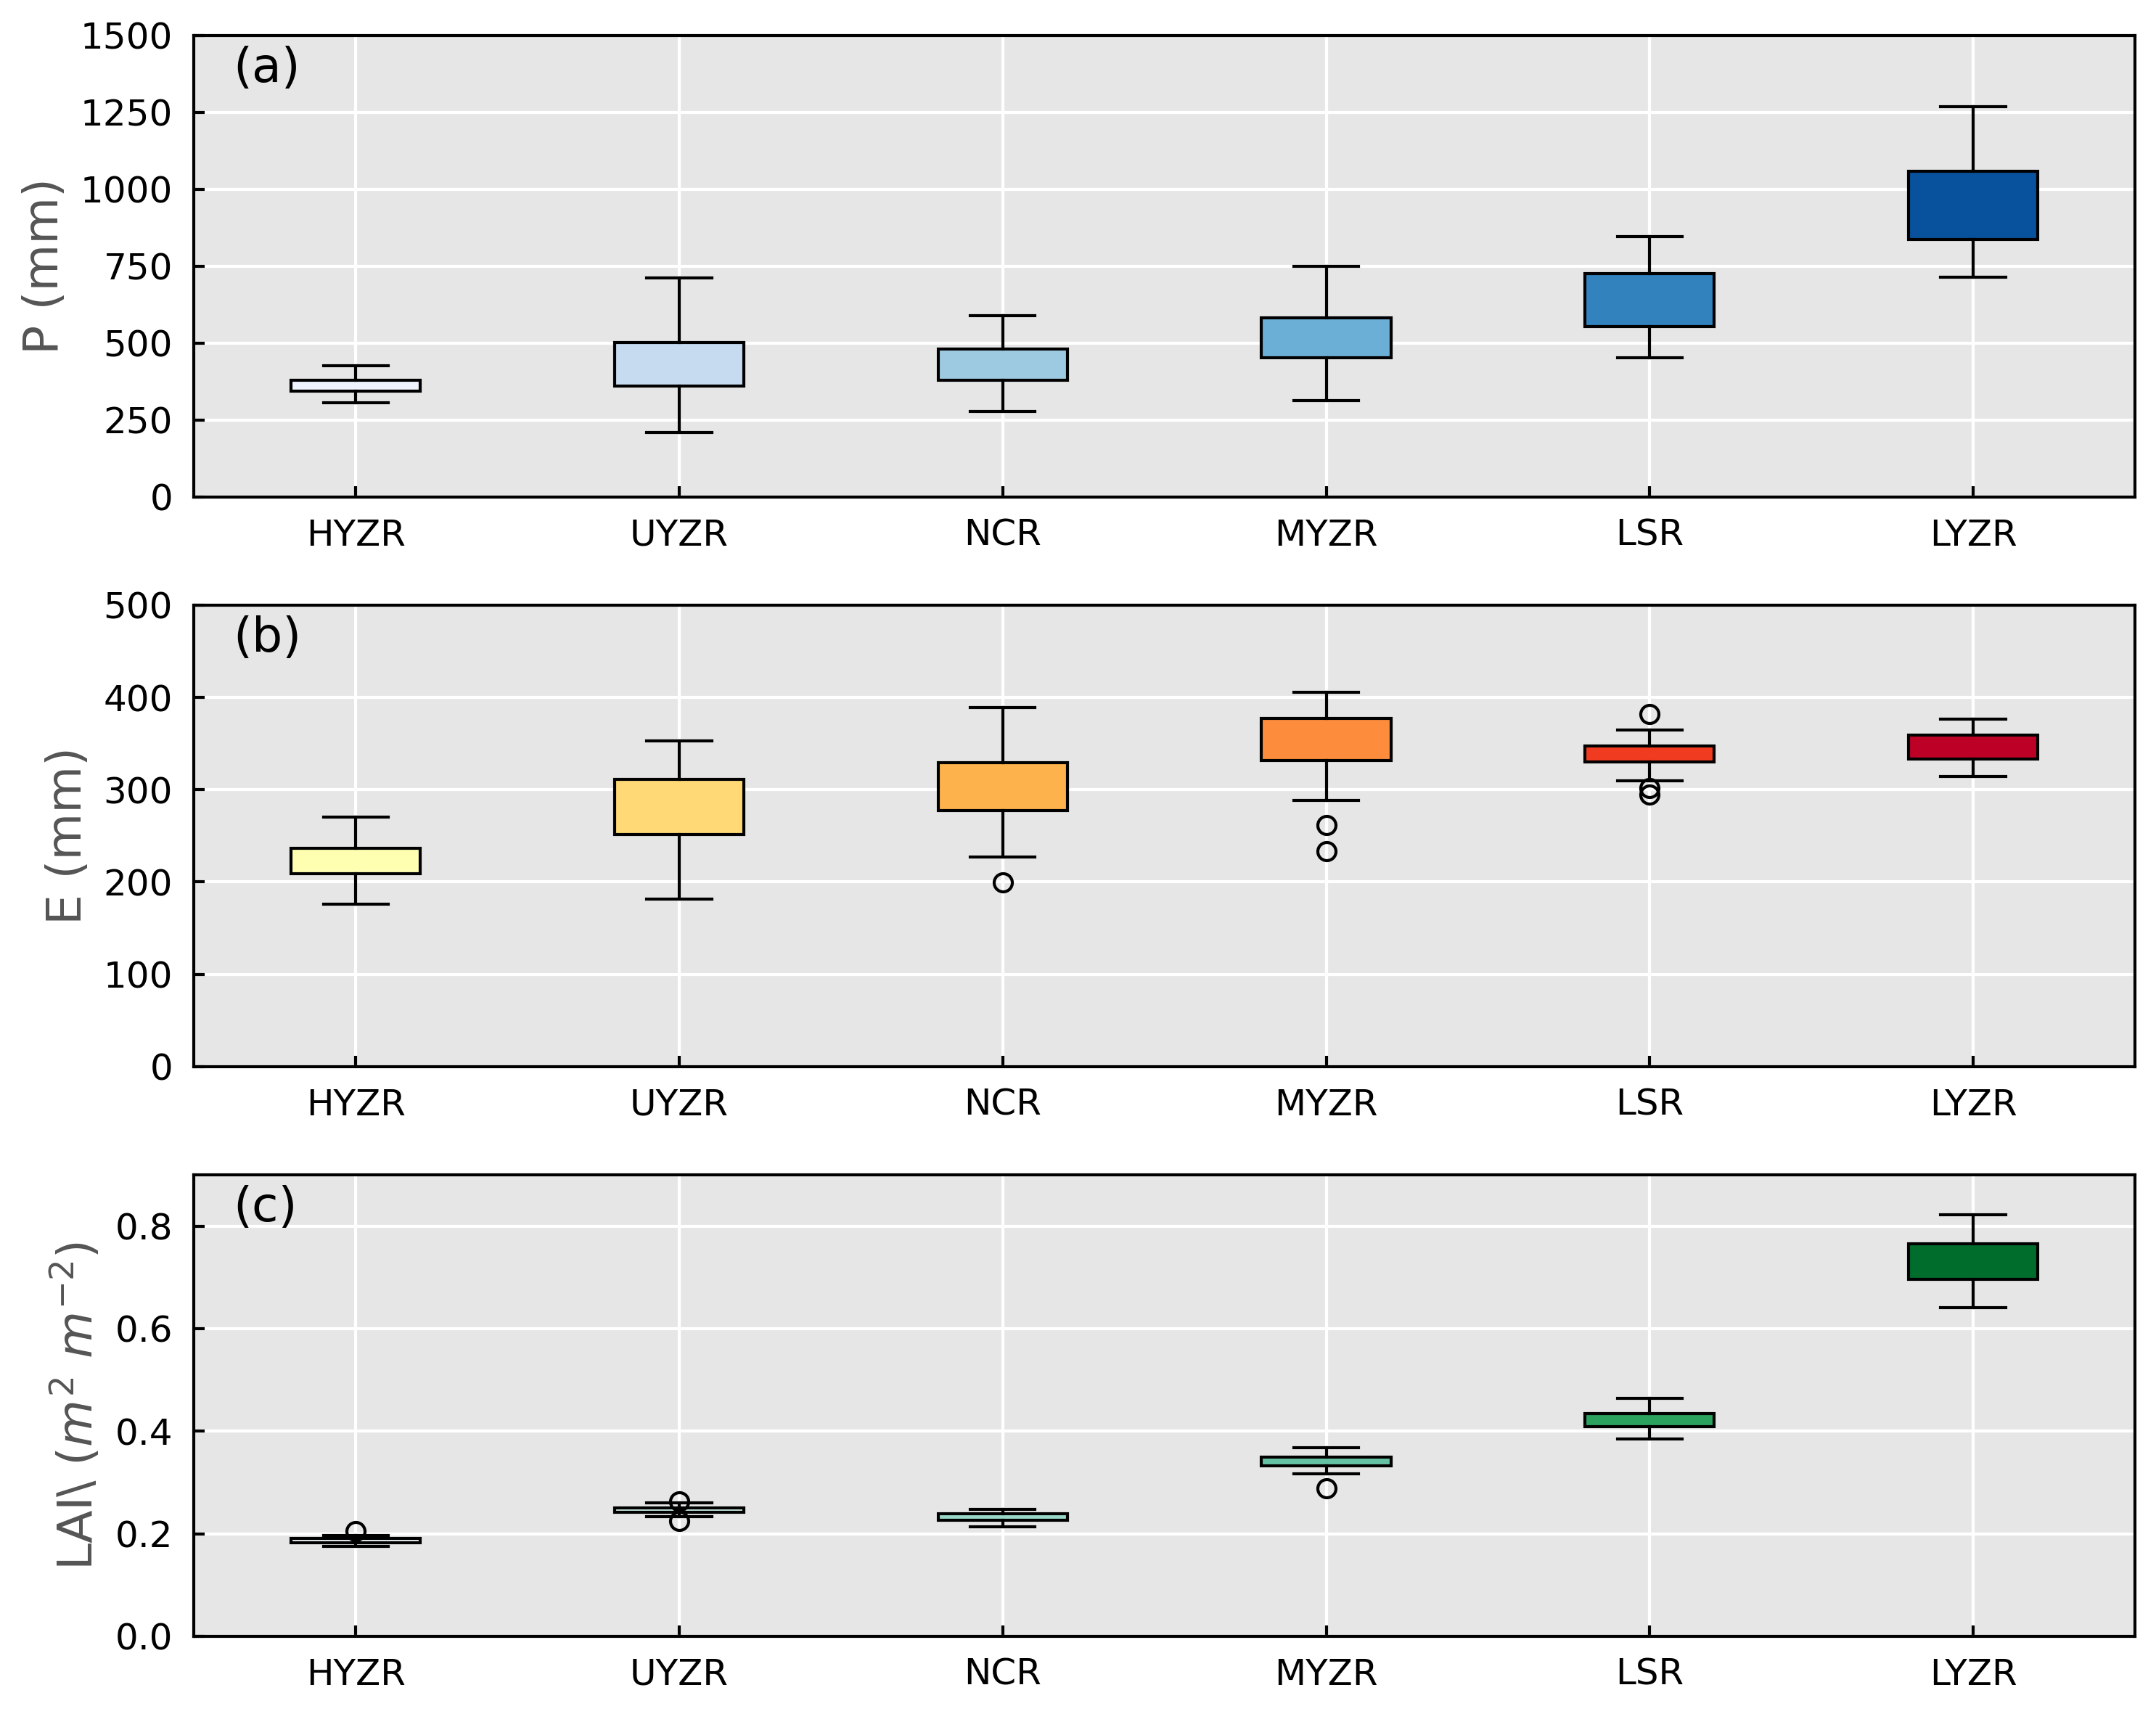
\includegraphics[width=\textwidth]{02-figures/climate-means.png}
    \caption{The distribution of (a) precipitation (P), (b) evaporation (E), and (c) Leaf Area Index (LAI) during 1982--2013 in the entire UBR basin. Black "x" signals show the mean value.}
    \label{figS:climate means}
\end{figure*}

\begin{figure*}[ht]
    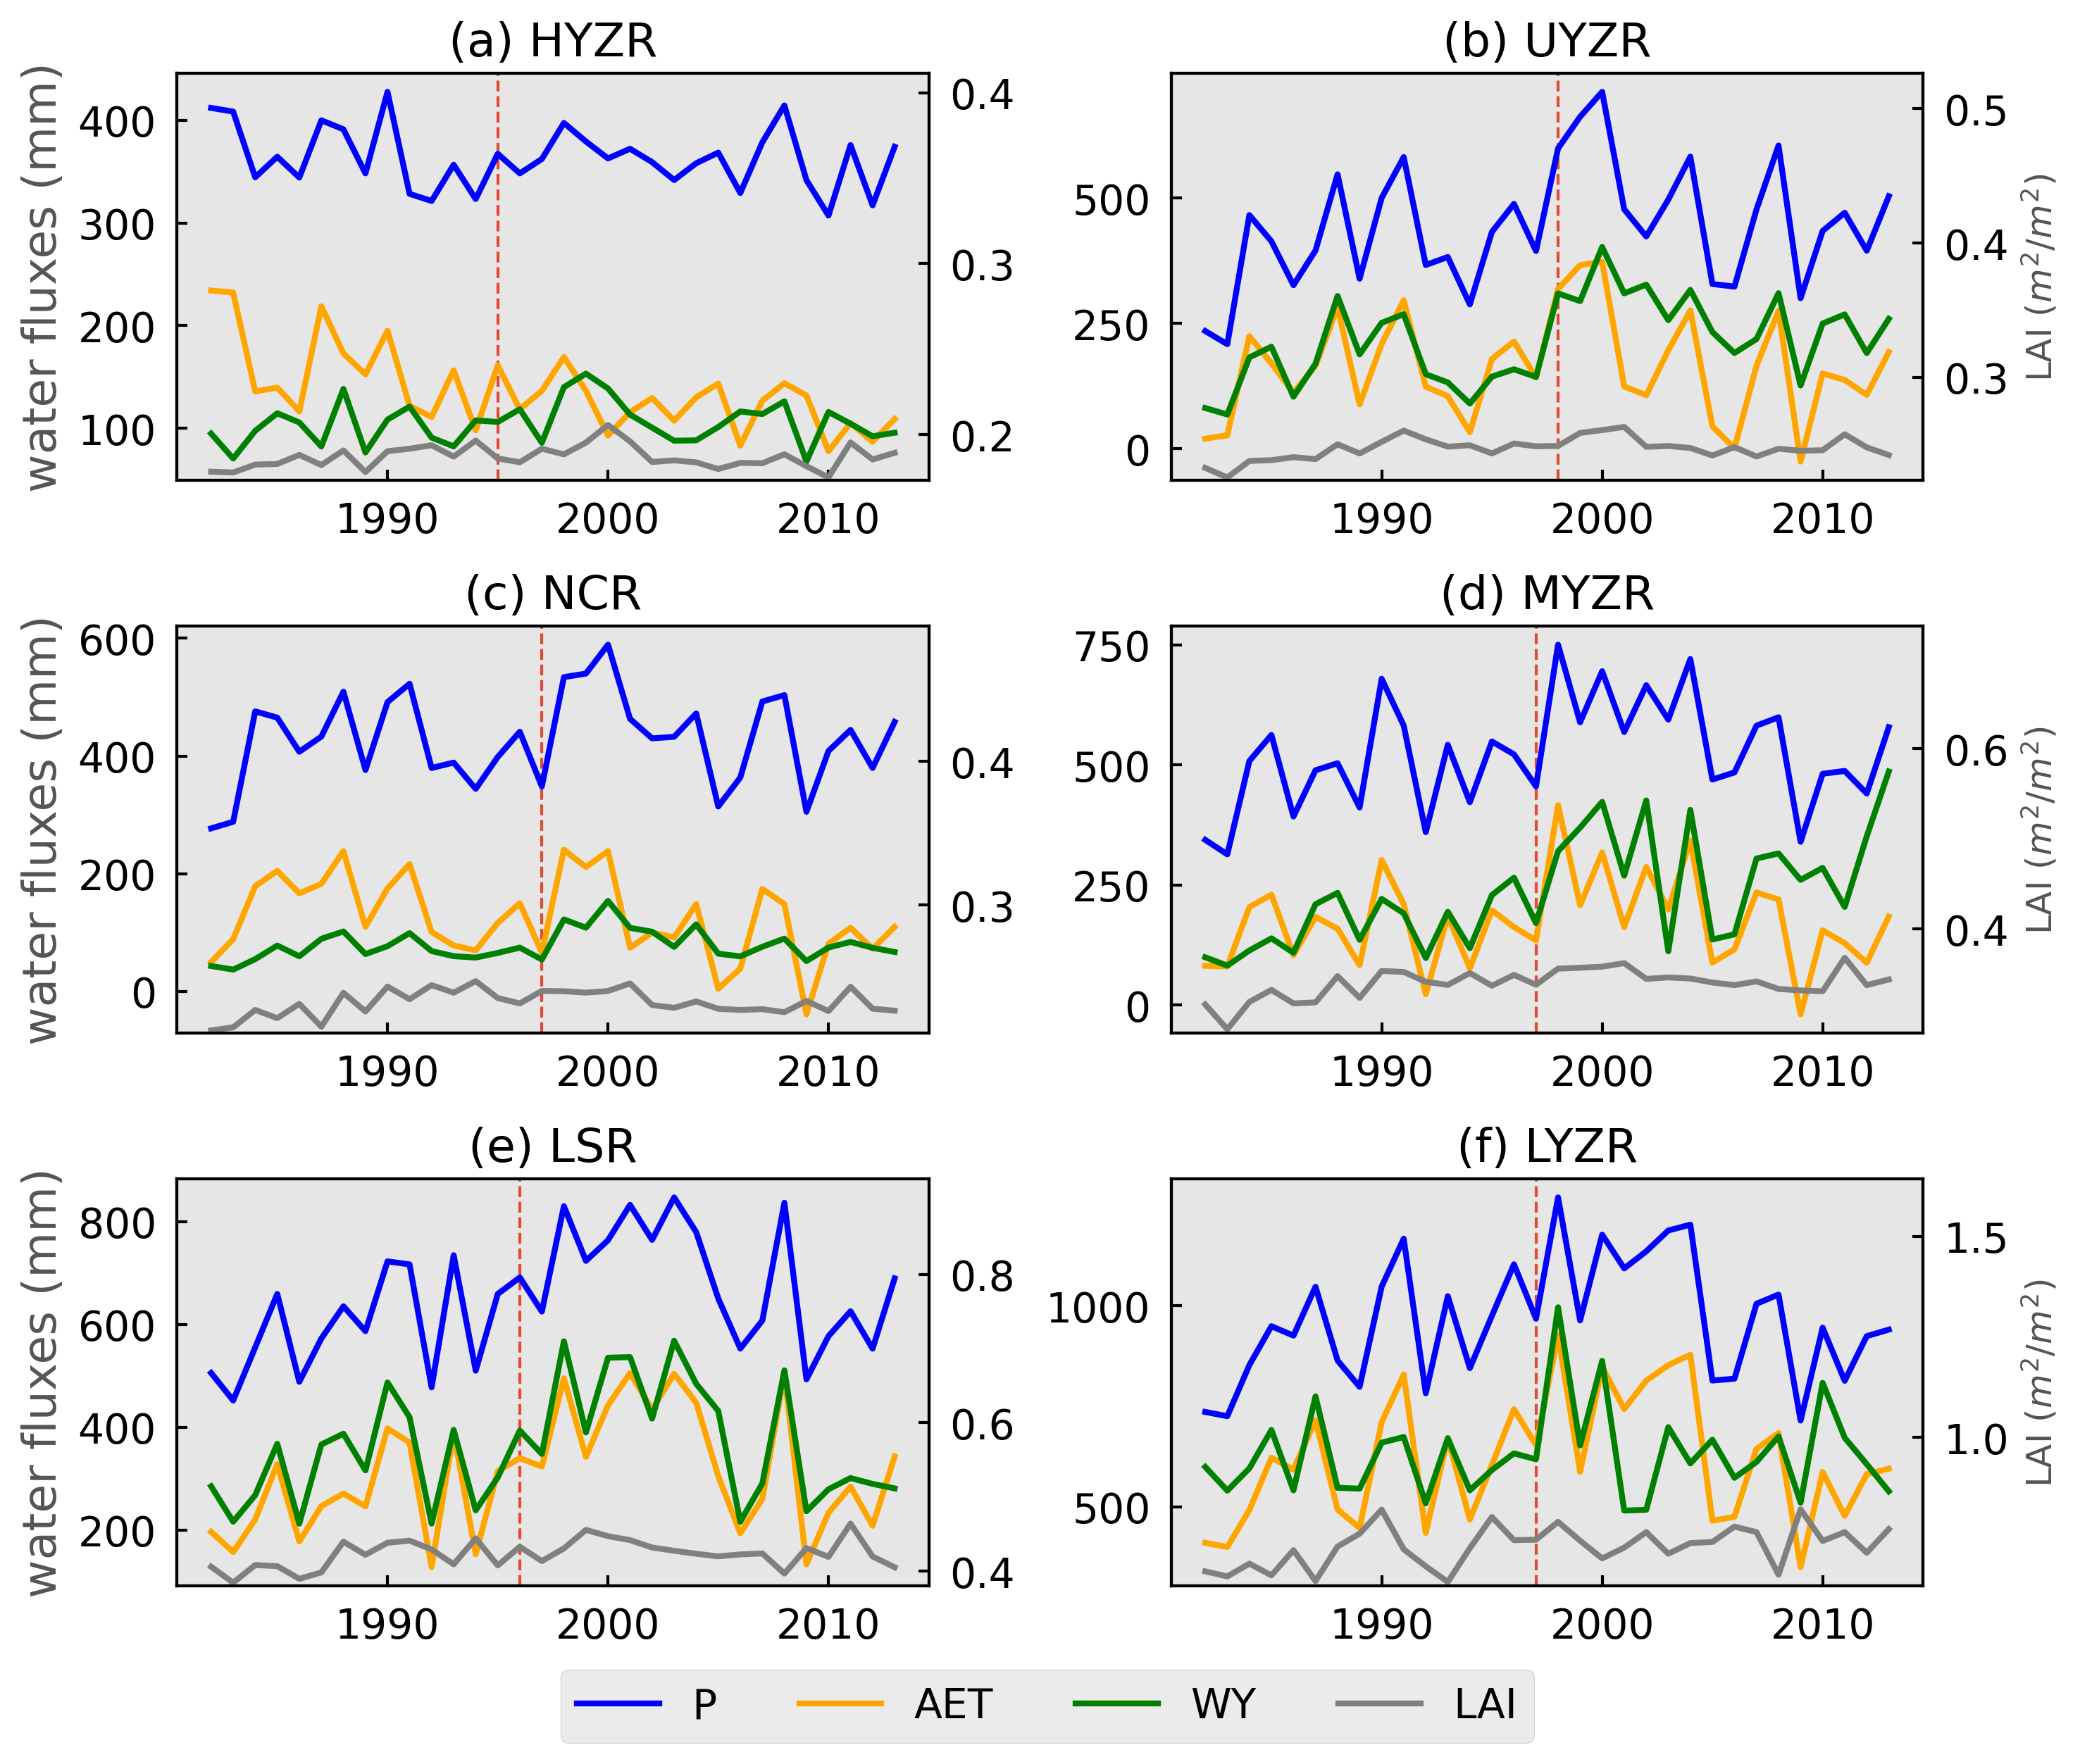
\includegraphics[width=\textwidth]{02-figures/time-series.png}
    \caption{The temporal changes of precipitation (P, blue line), evaporation (E, orange line), and water yield (WY, green line) and Leaf Area Index (LAI, grey line) during 1982--2013 in the entire UBR basin. The vertical line indicates the turning point in WY.}
    \label{figS:time series}
\end{figure*}

\begin{figure*}[ht]
    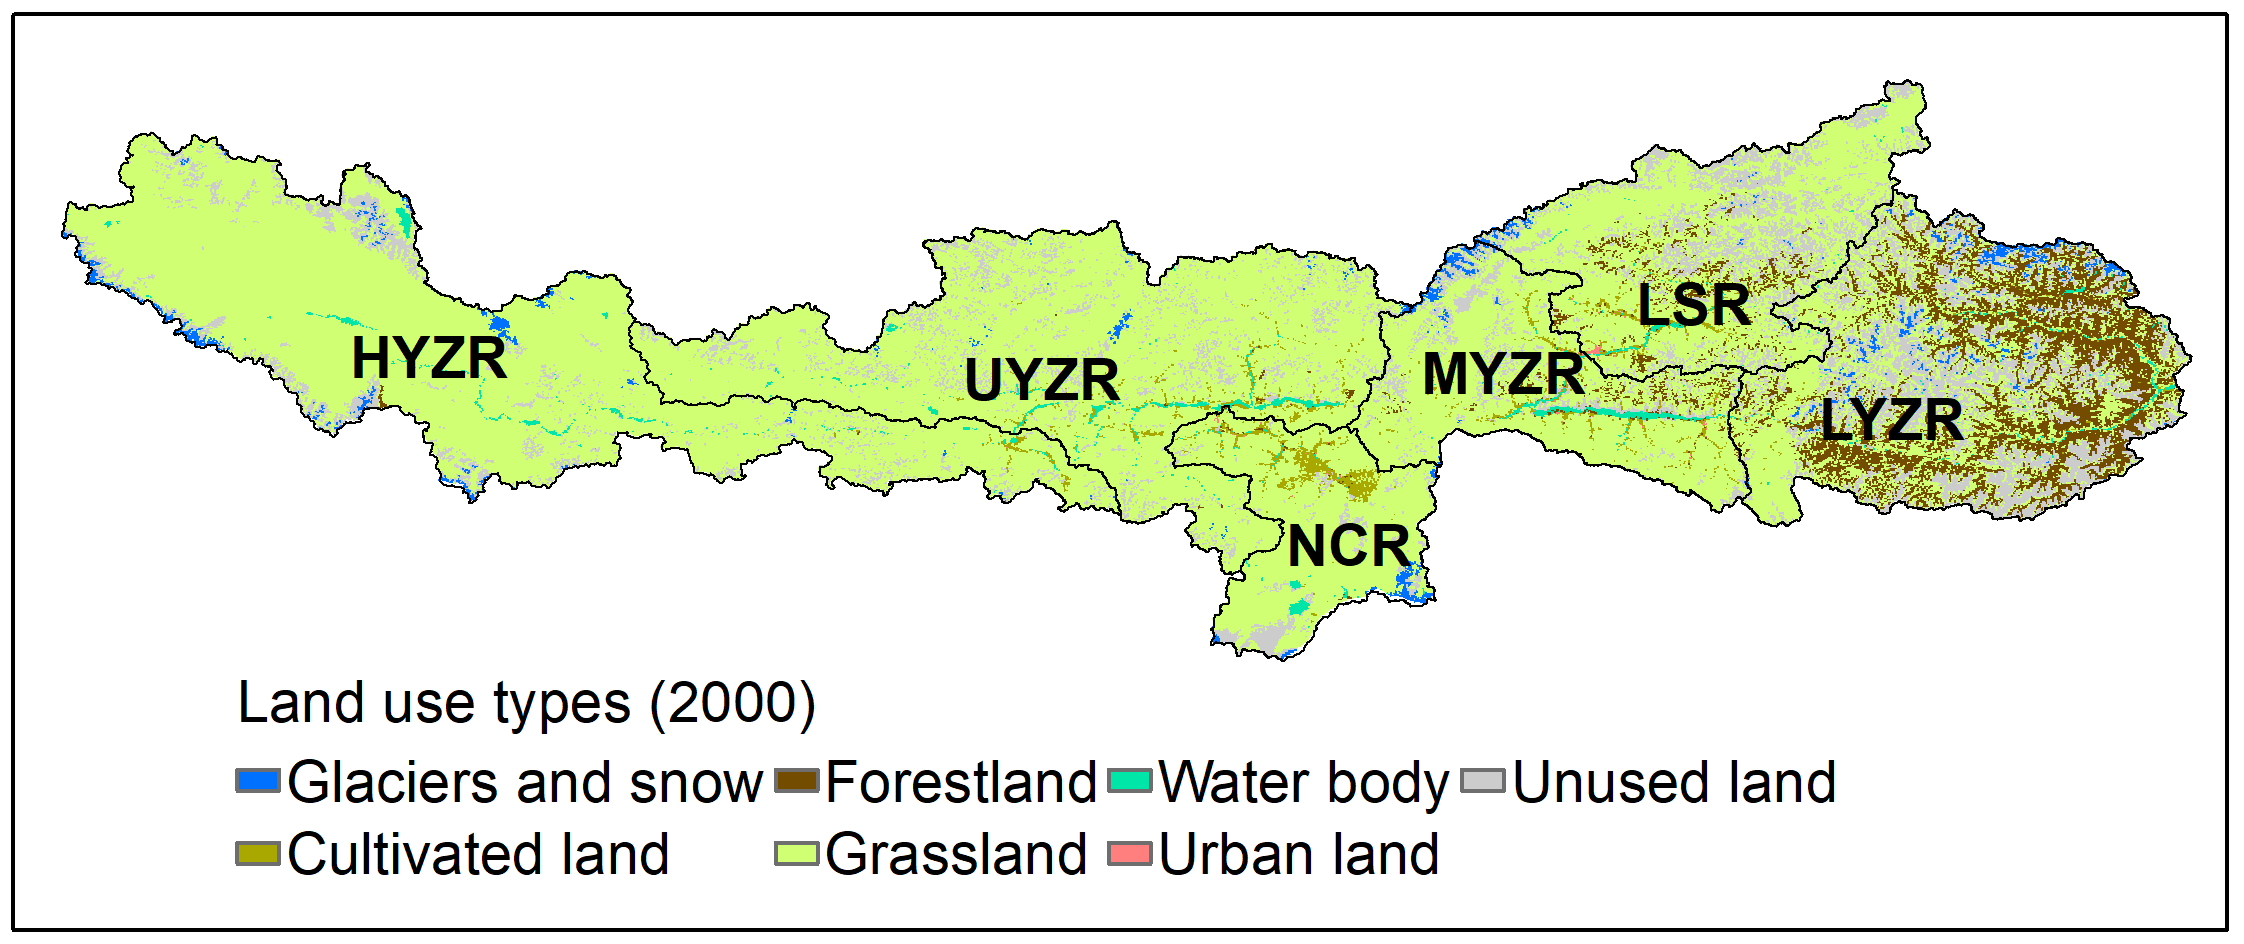
\includegraphics[width=\textwidth]{02-figures/lucc2000.png}
    \caption{The land use types in 2000 in the UBR basin.}
    \label{figS:lucc}
\end{figure*}

\begin{figure*}[ht]
    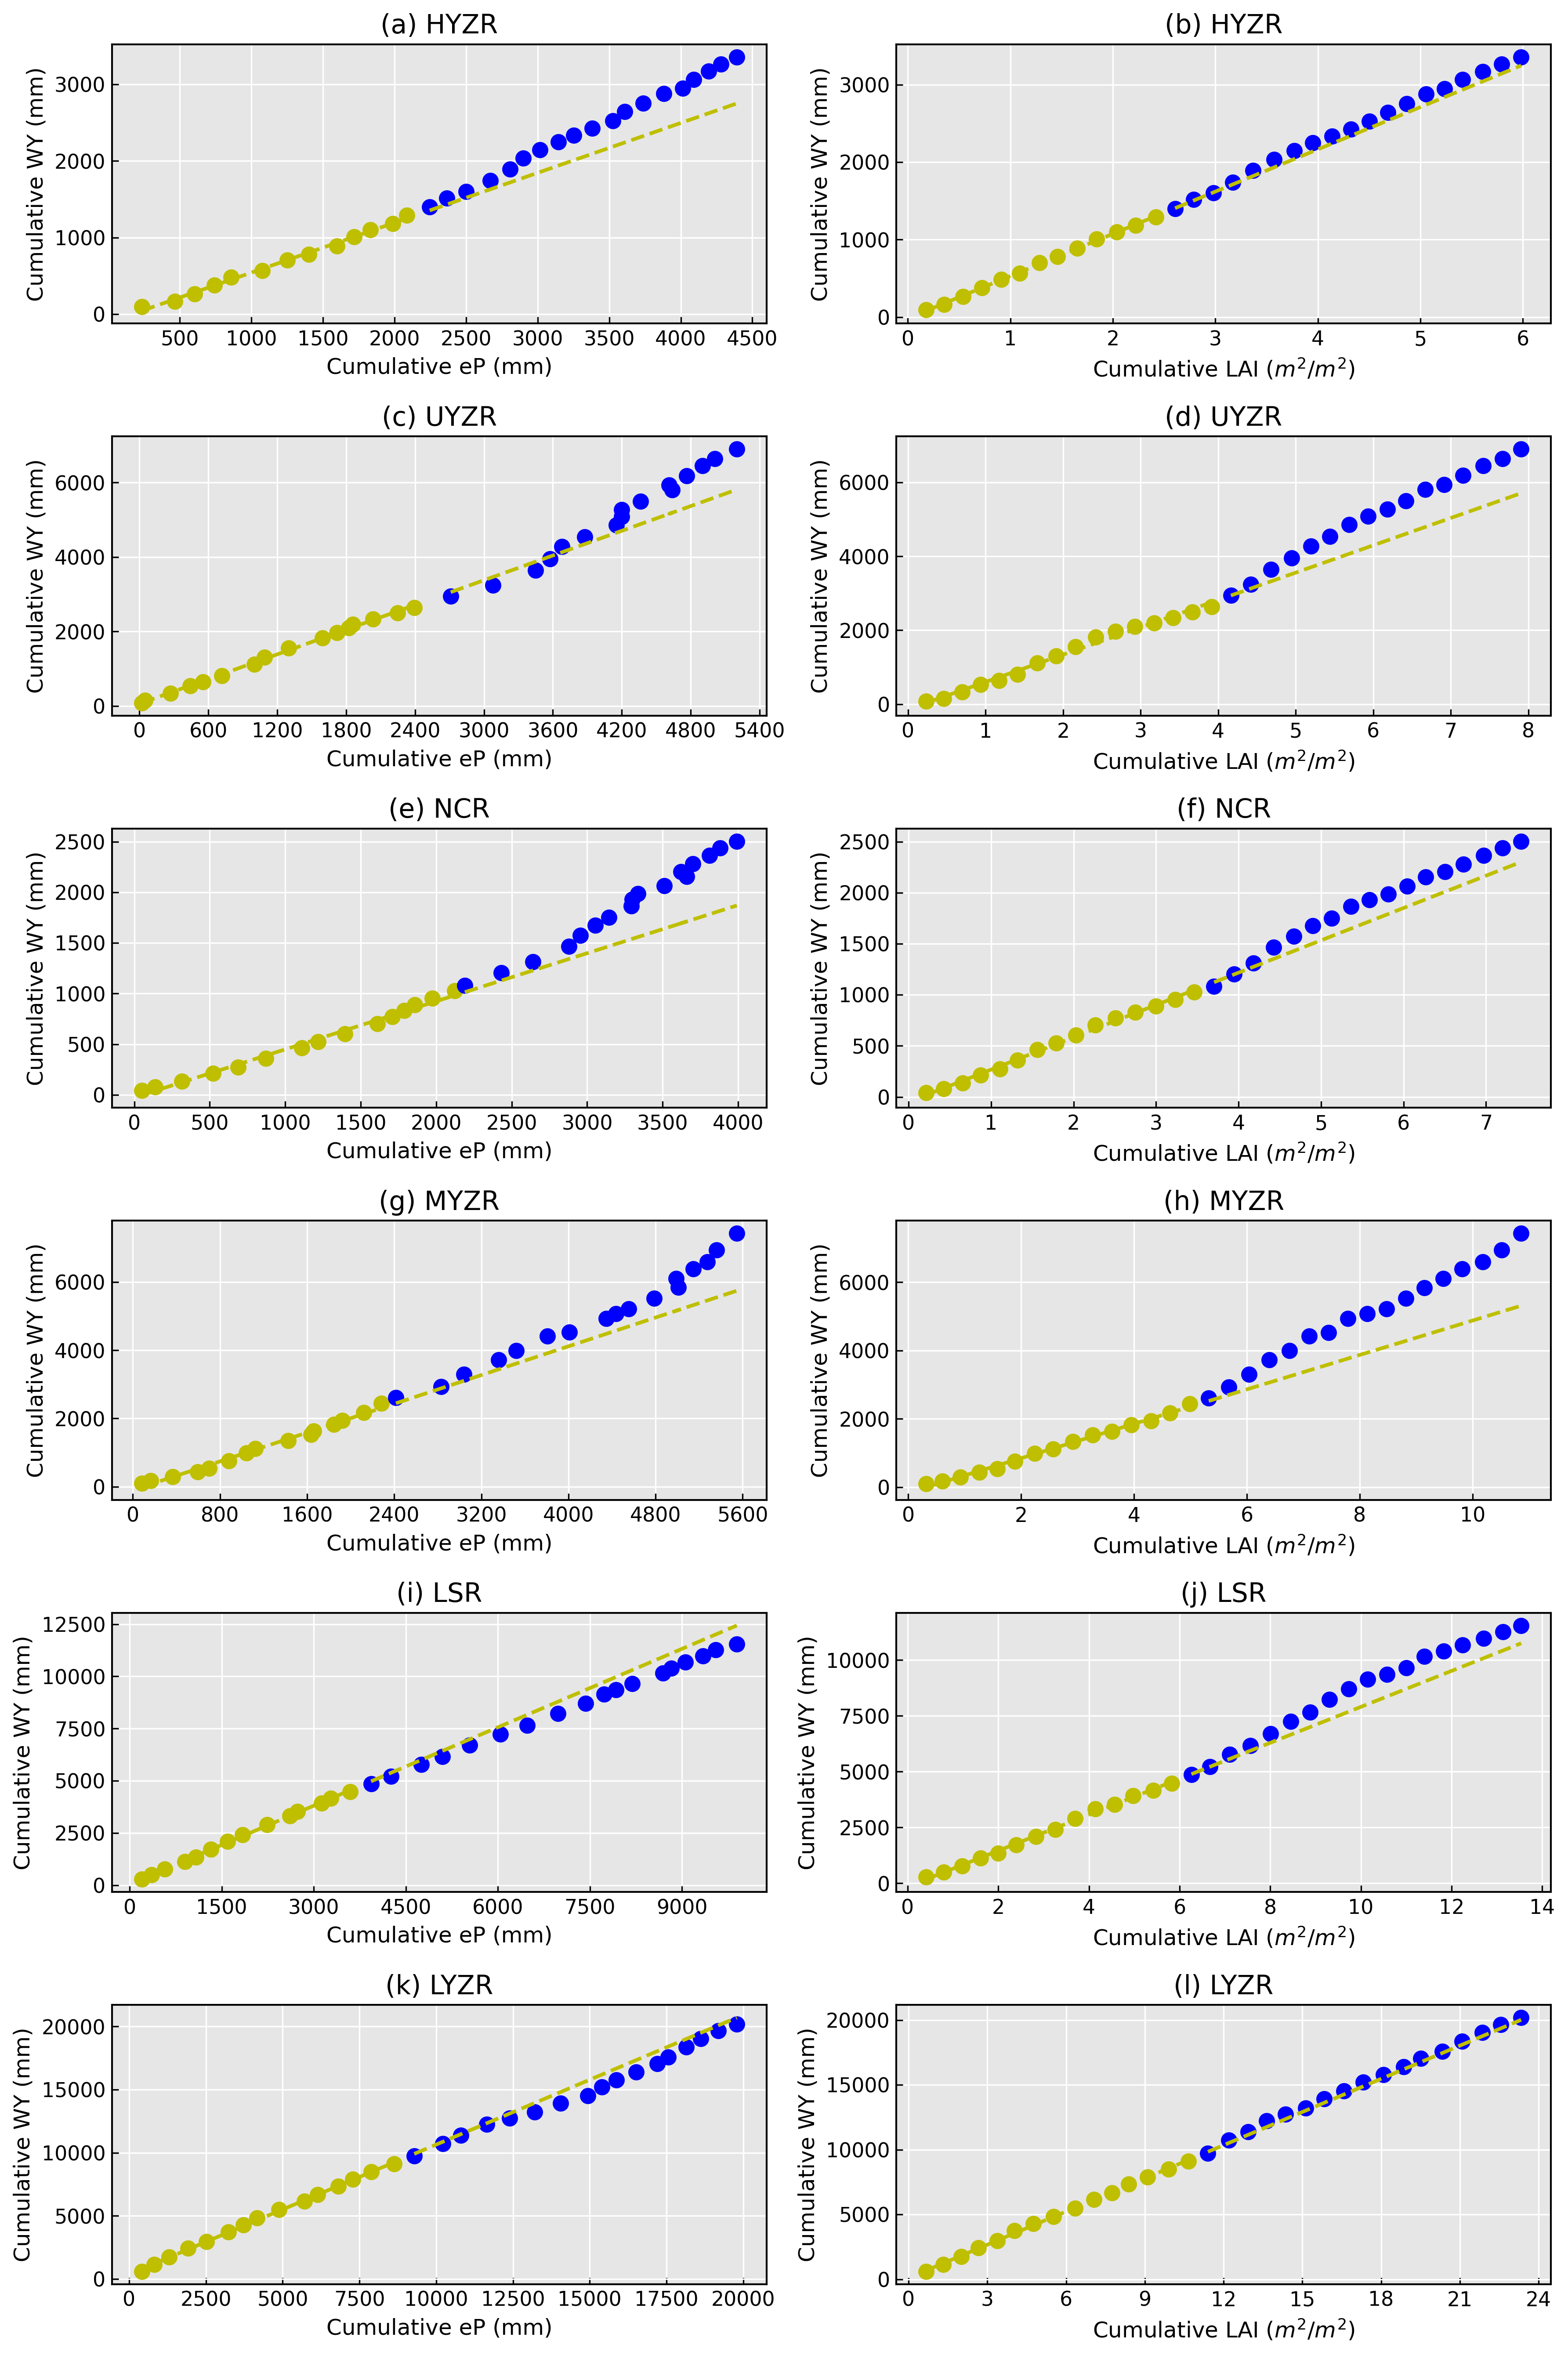
\includegraphics[width=0.75\textwidth]{02-figures/DMC-predictive-lines.png}
    \caption{Double mass curves in the entire UBR basin. The left panel (a+c+e+g+i+k) shows the double mass curve between cumulative eP (x-axis) and WY (y-axis), and the right panel (b+d+f+h+j+l) shows the double mass between cumulative LAI (x-axis) and WY (y-axis). 
    The color of points represents the period before (yellow) and after (blue) Tp.
    The dash line indicates the predictions by inputting cumulative eP or LAI in Equation (2) or (3) in main text.}
    \label{figS:DMC}
\end{figure*}

\begin{figure*}[ht]
    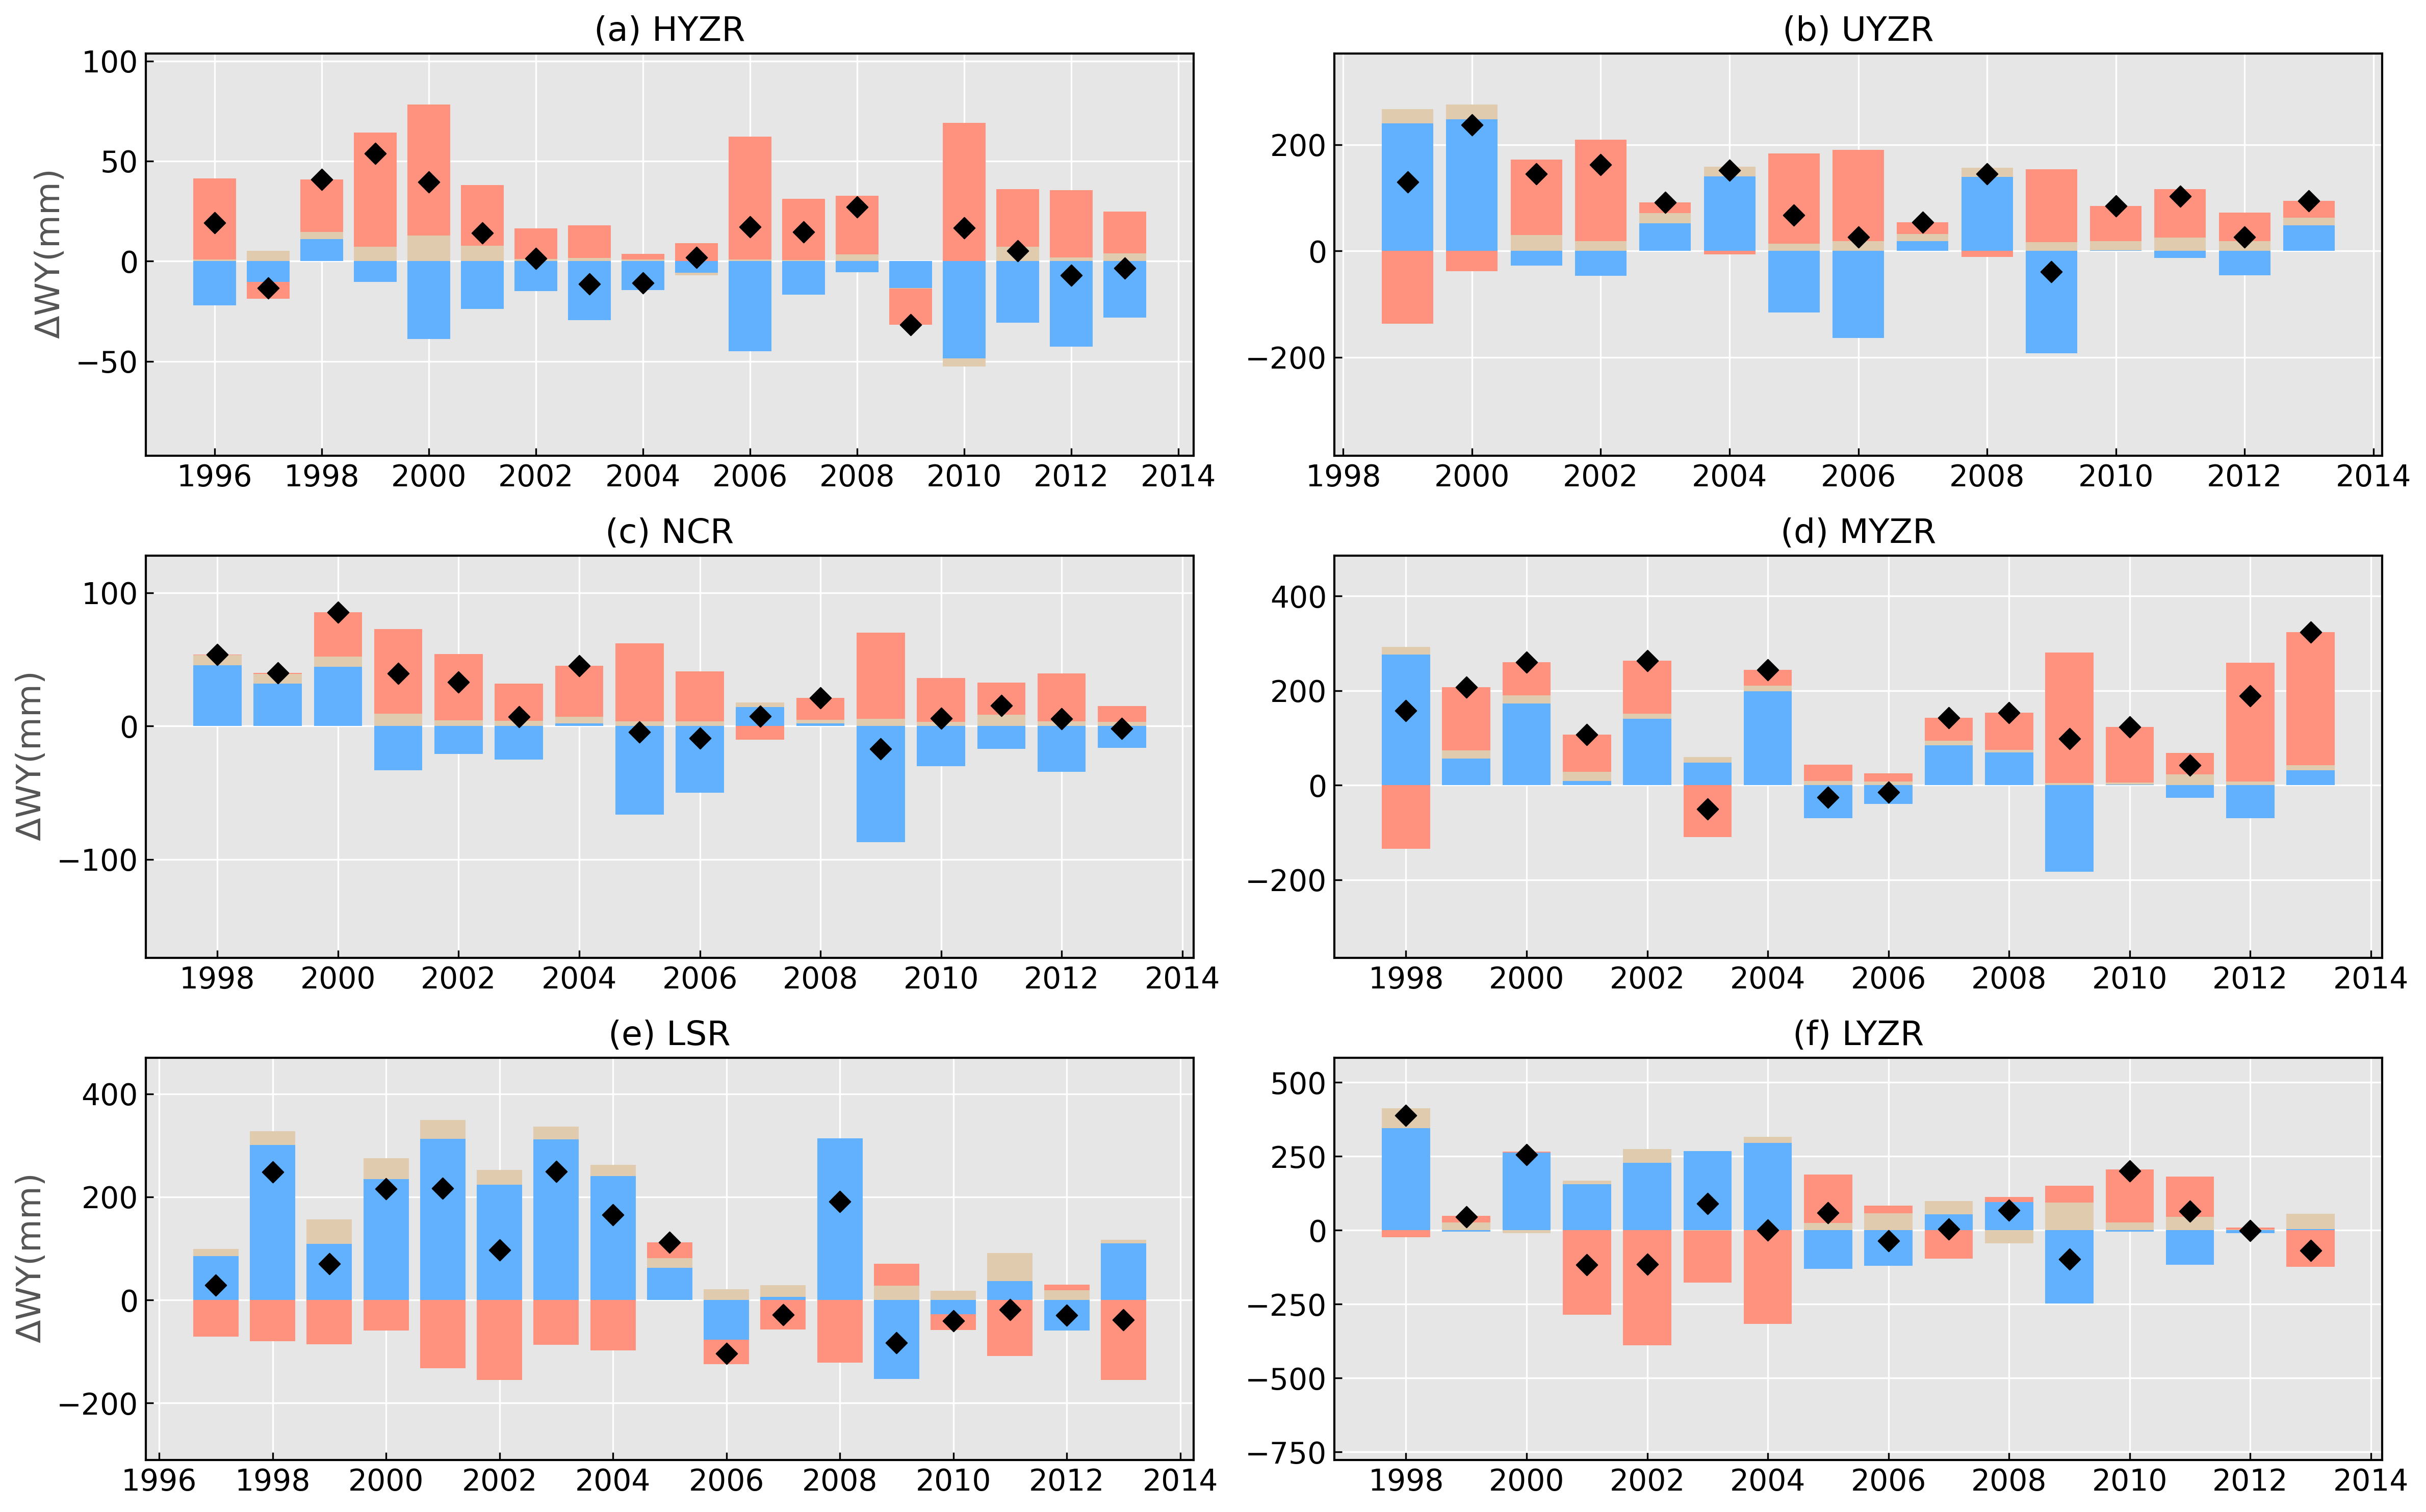
\includegraphics[width=\textwidth]{02-figures/water-yield-deviation.png}
    \caption
    {Time series after Tp of total water yield deviation ($\Delta WY_s(t)$, black diamond), consisting of water yield deviation from climate ($\Delta WY_c$, blue bar), vegetation ($\Delta WY_v$, tan bar), and cryosphere ($\Delta WY_g$, red bar).}
    \label{fig:attribution-results}
\end{figure*}

\begin{figure*}[ht]
    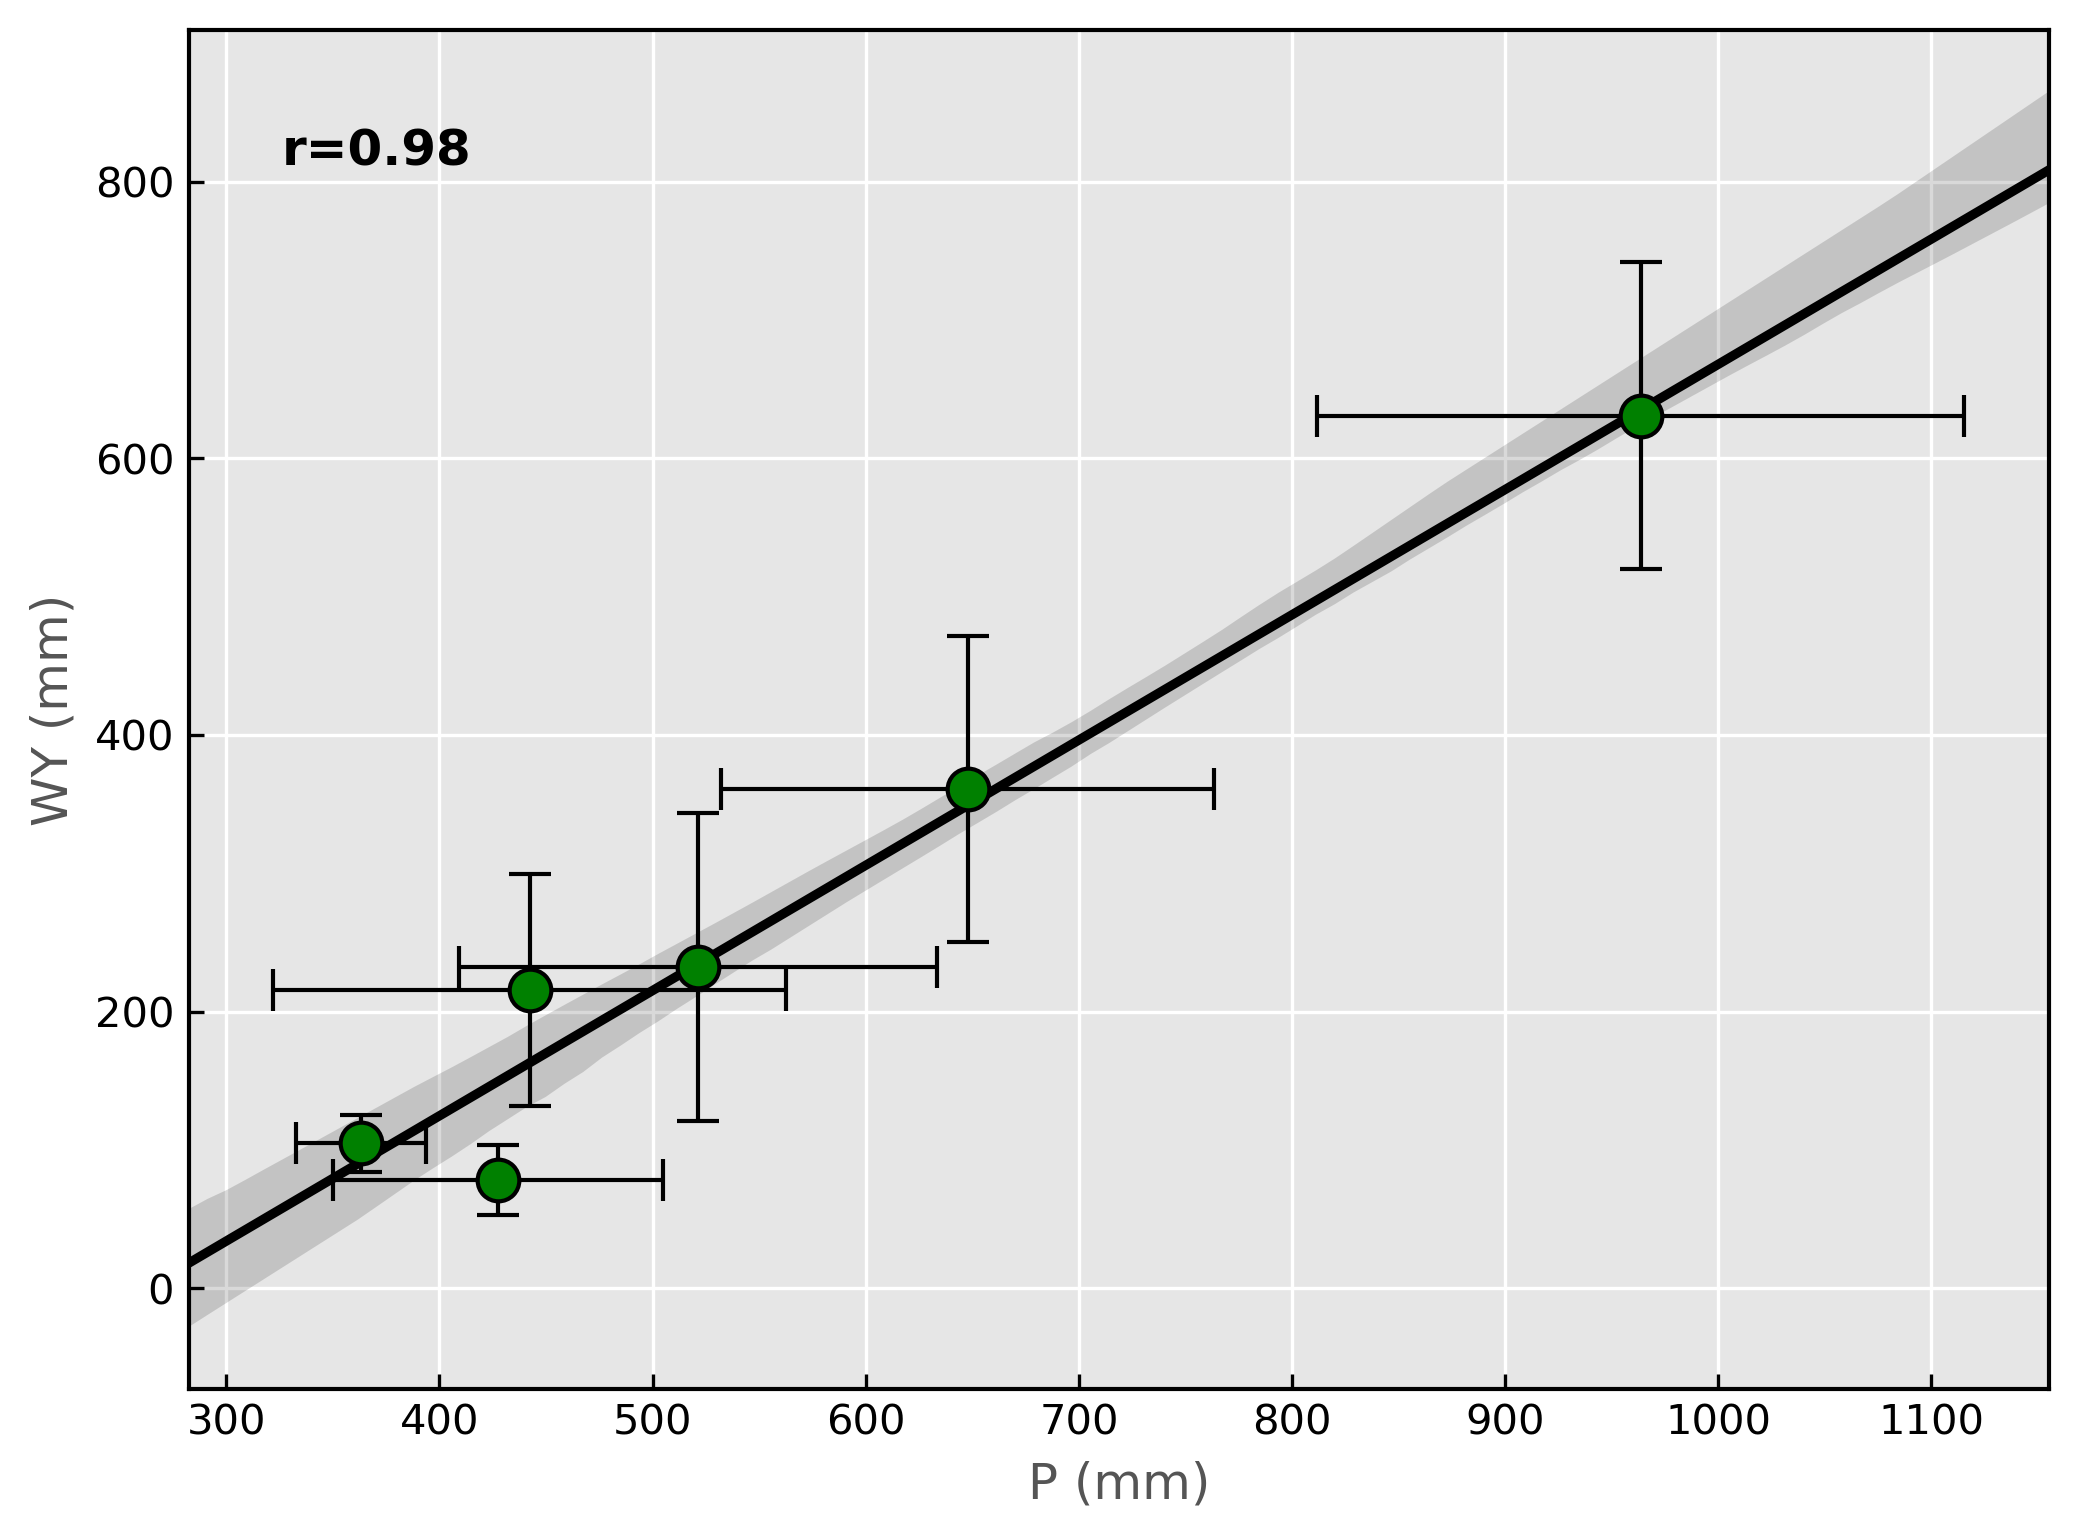
\includegraphics[width=\textwidth]{02-figures/pre-and-water-yield.png}
    \caption{The relationship between precipitation (P) and water yield
    (WY) in the entire UBR basin. The error bar represents one standard deviation. 
    The shading area indicates the 95\% confidence interval of the linear fitting.}
    \label{figS:P-and-WY}
\end{figure*}

\begin{figure*}[ht]
    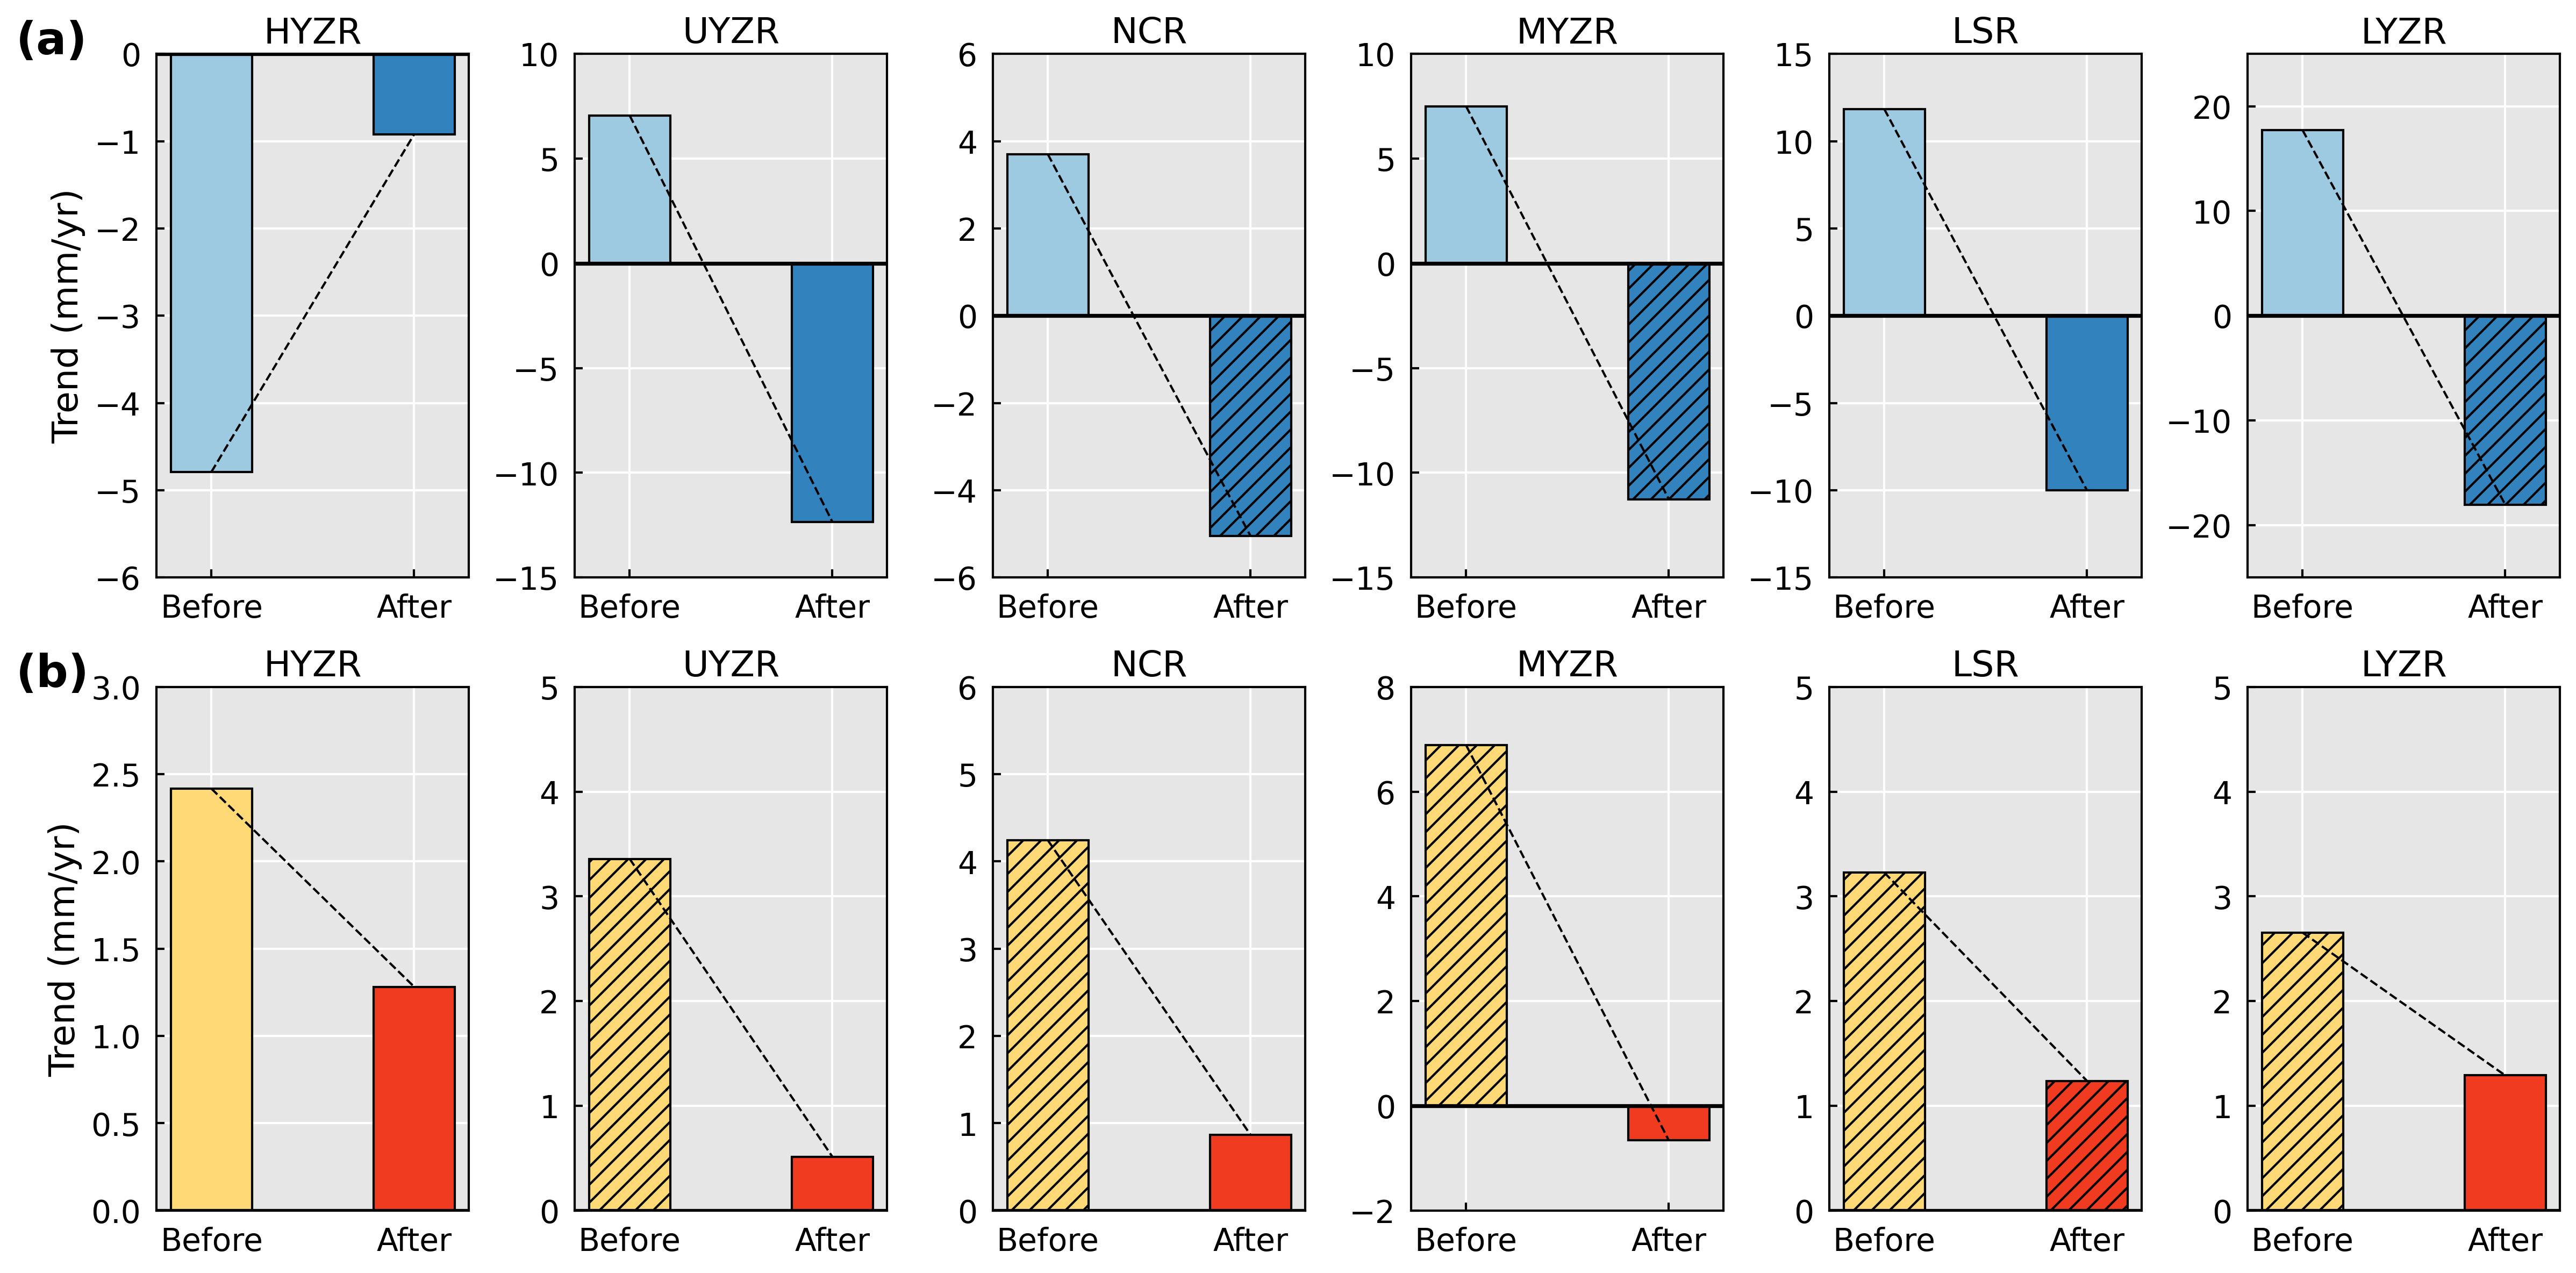
\includegraphics[width=\textwidth]{02-figures/P_AET_diections.png}
    \caption{Direction of precipitation (a) and evaporation (b) changes. 
    The black hatching represents the statistically significant trend (p < 0.05).
    The color of boxes represents the period before (light color) and after (dark color) Tp.}
    \label{figS:climate-directions}
\end{figure*}

\begin{figure*}[ht]
    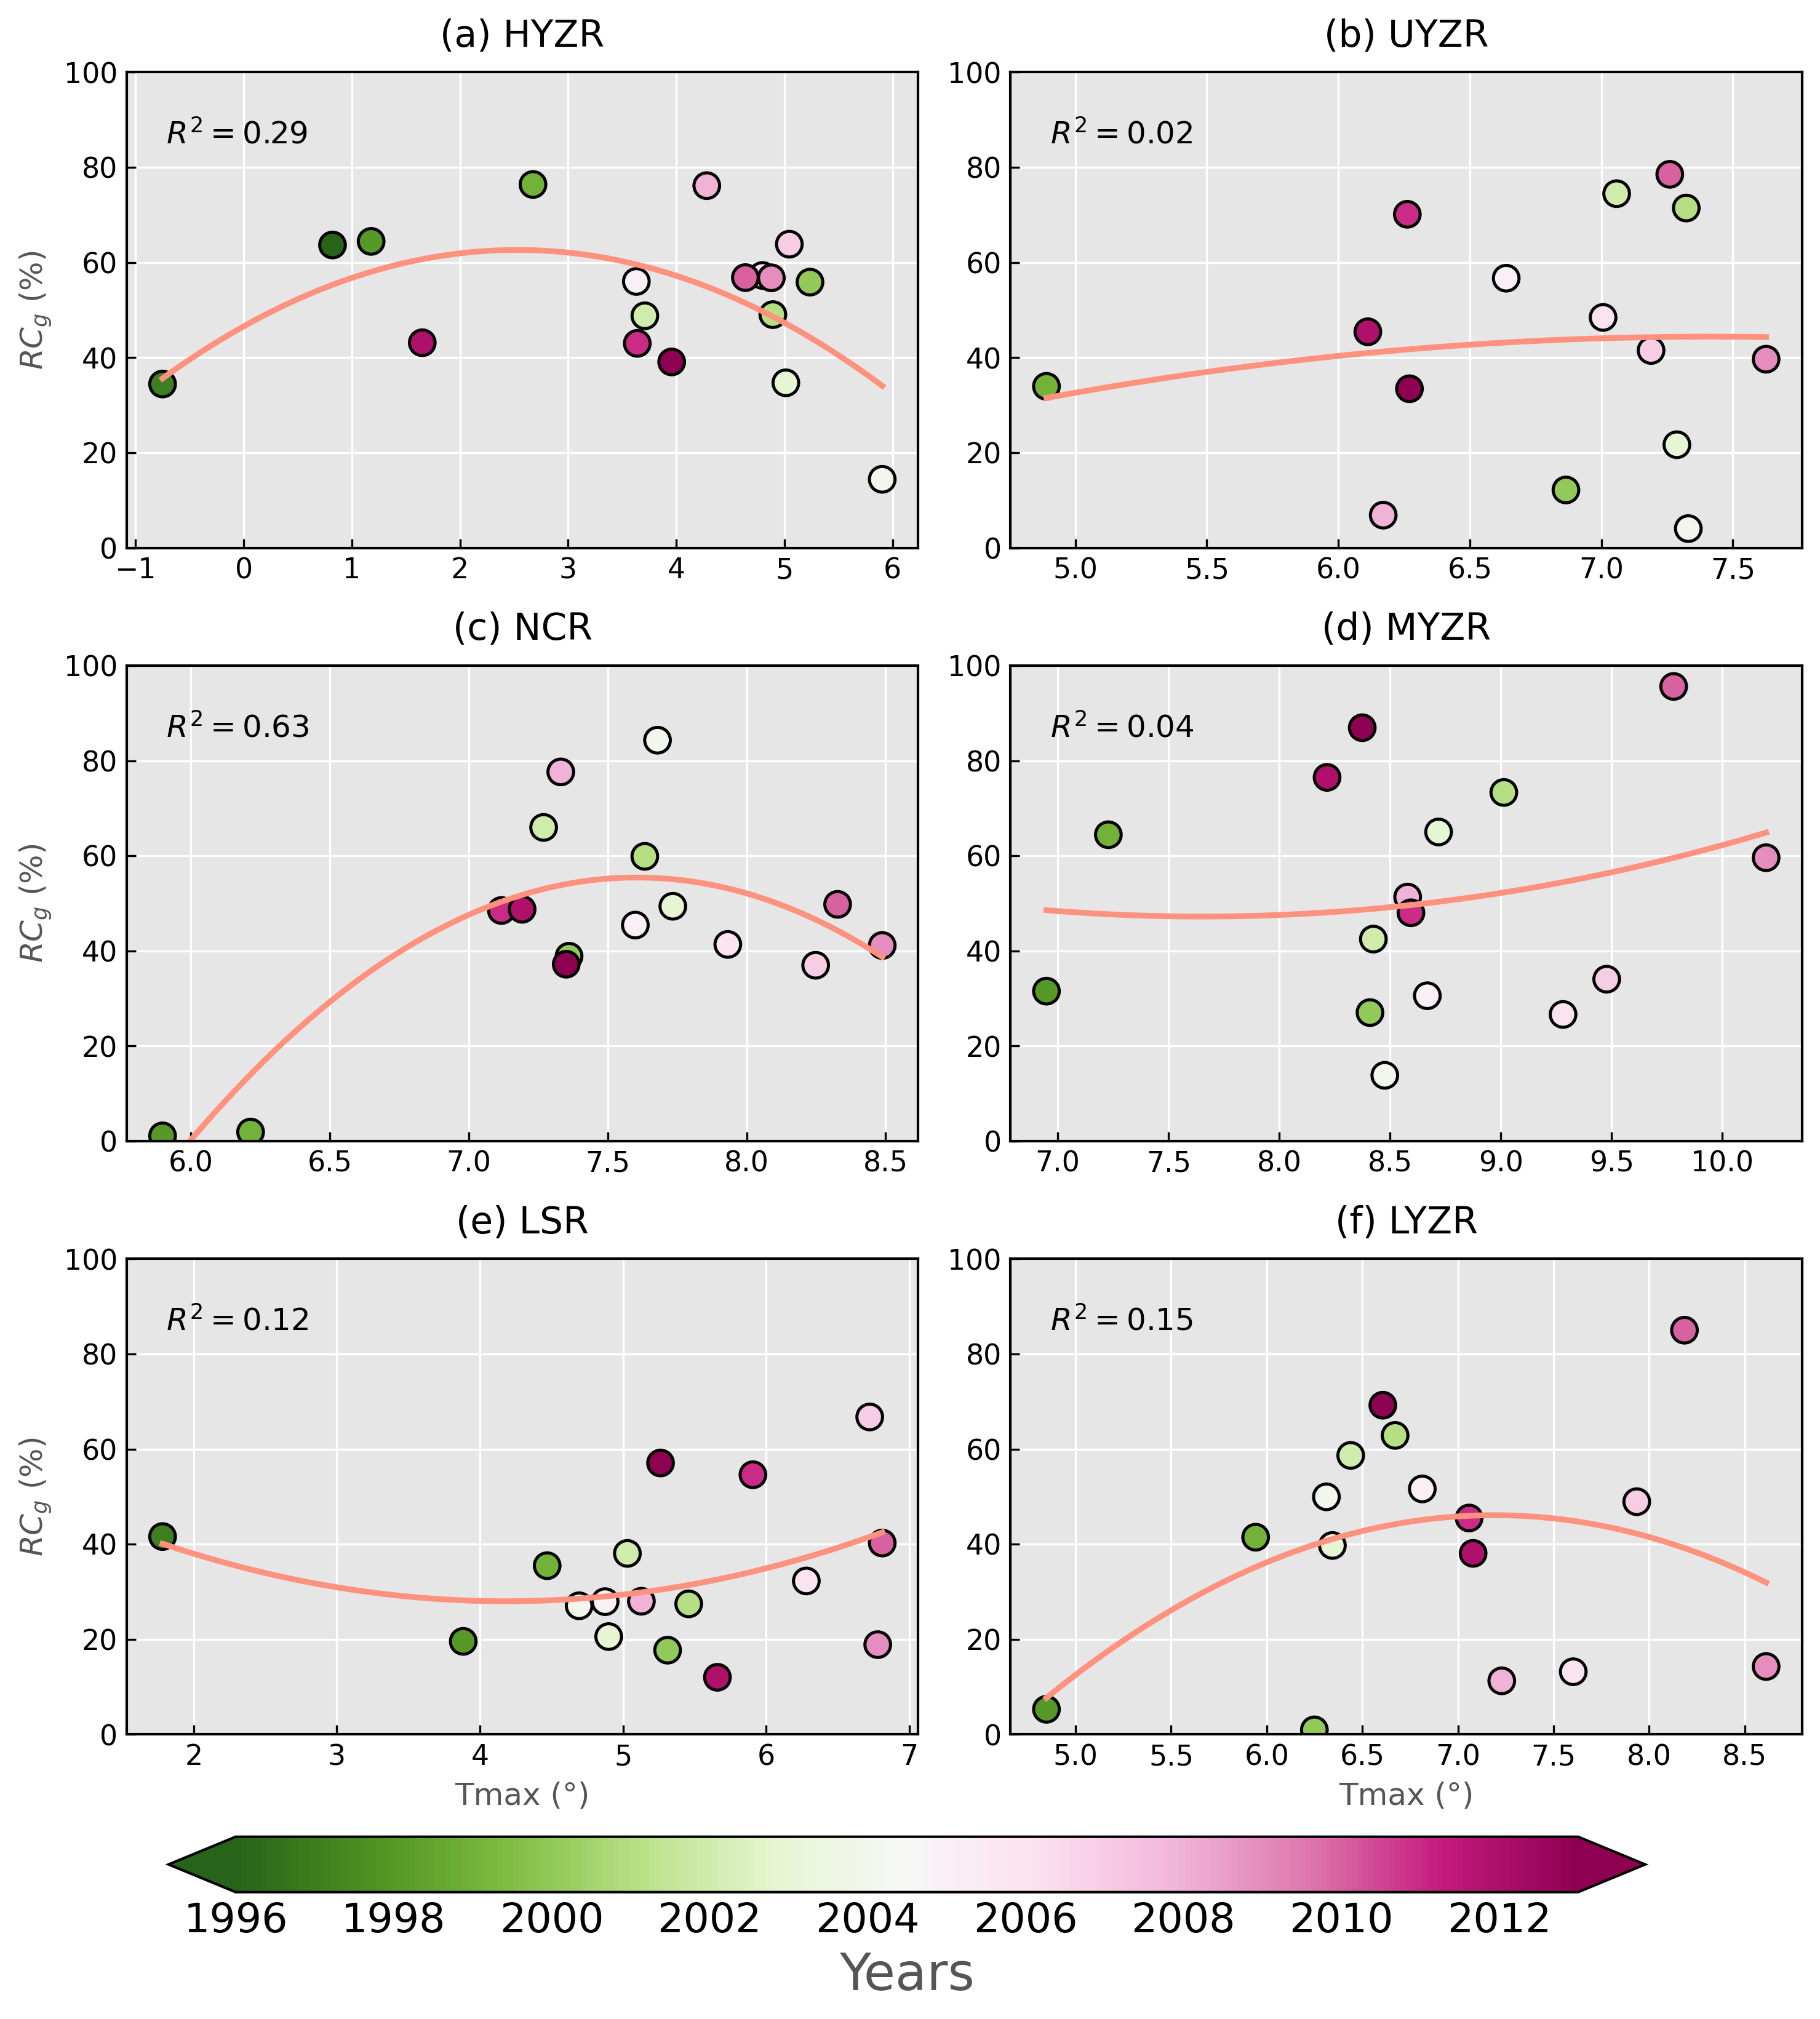
\includegraphics[width=\textwidth]{02-figures/peak-water-analysis.png}
    \caption{The relationship between cryospheric contributions to water yield deviations ($RC_g(t)$, see Data and Methods) and annual mean 2 m maximum air temperature ($T_{max}$) using the polynomial fitting. 
    The colorbar indicates the years after Tp in individual basins. 
    R square here used to evaluate the fitting goodness is labelled in each panel.}
    \label{figS:warming-and-cryosphere}
\end{figure*}

\begin{figure*}[ht]
    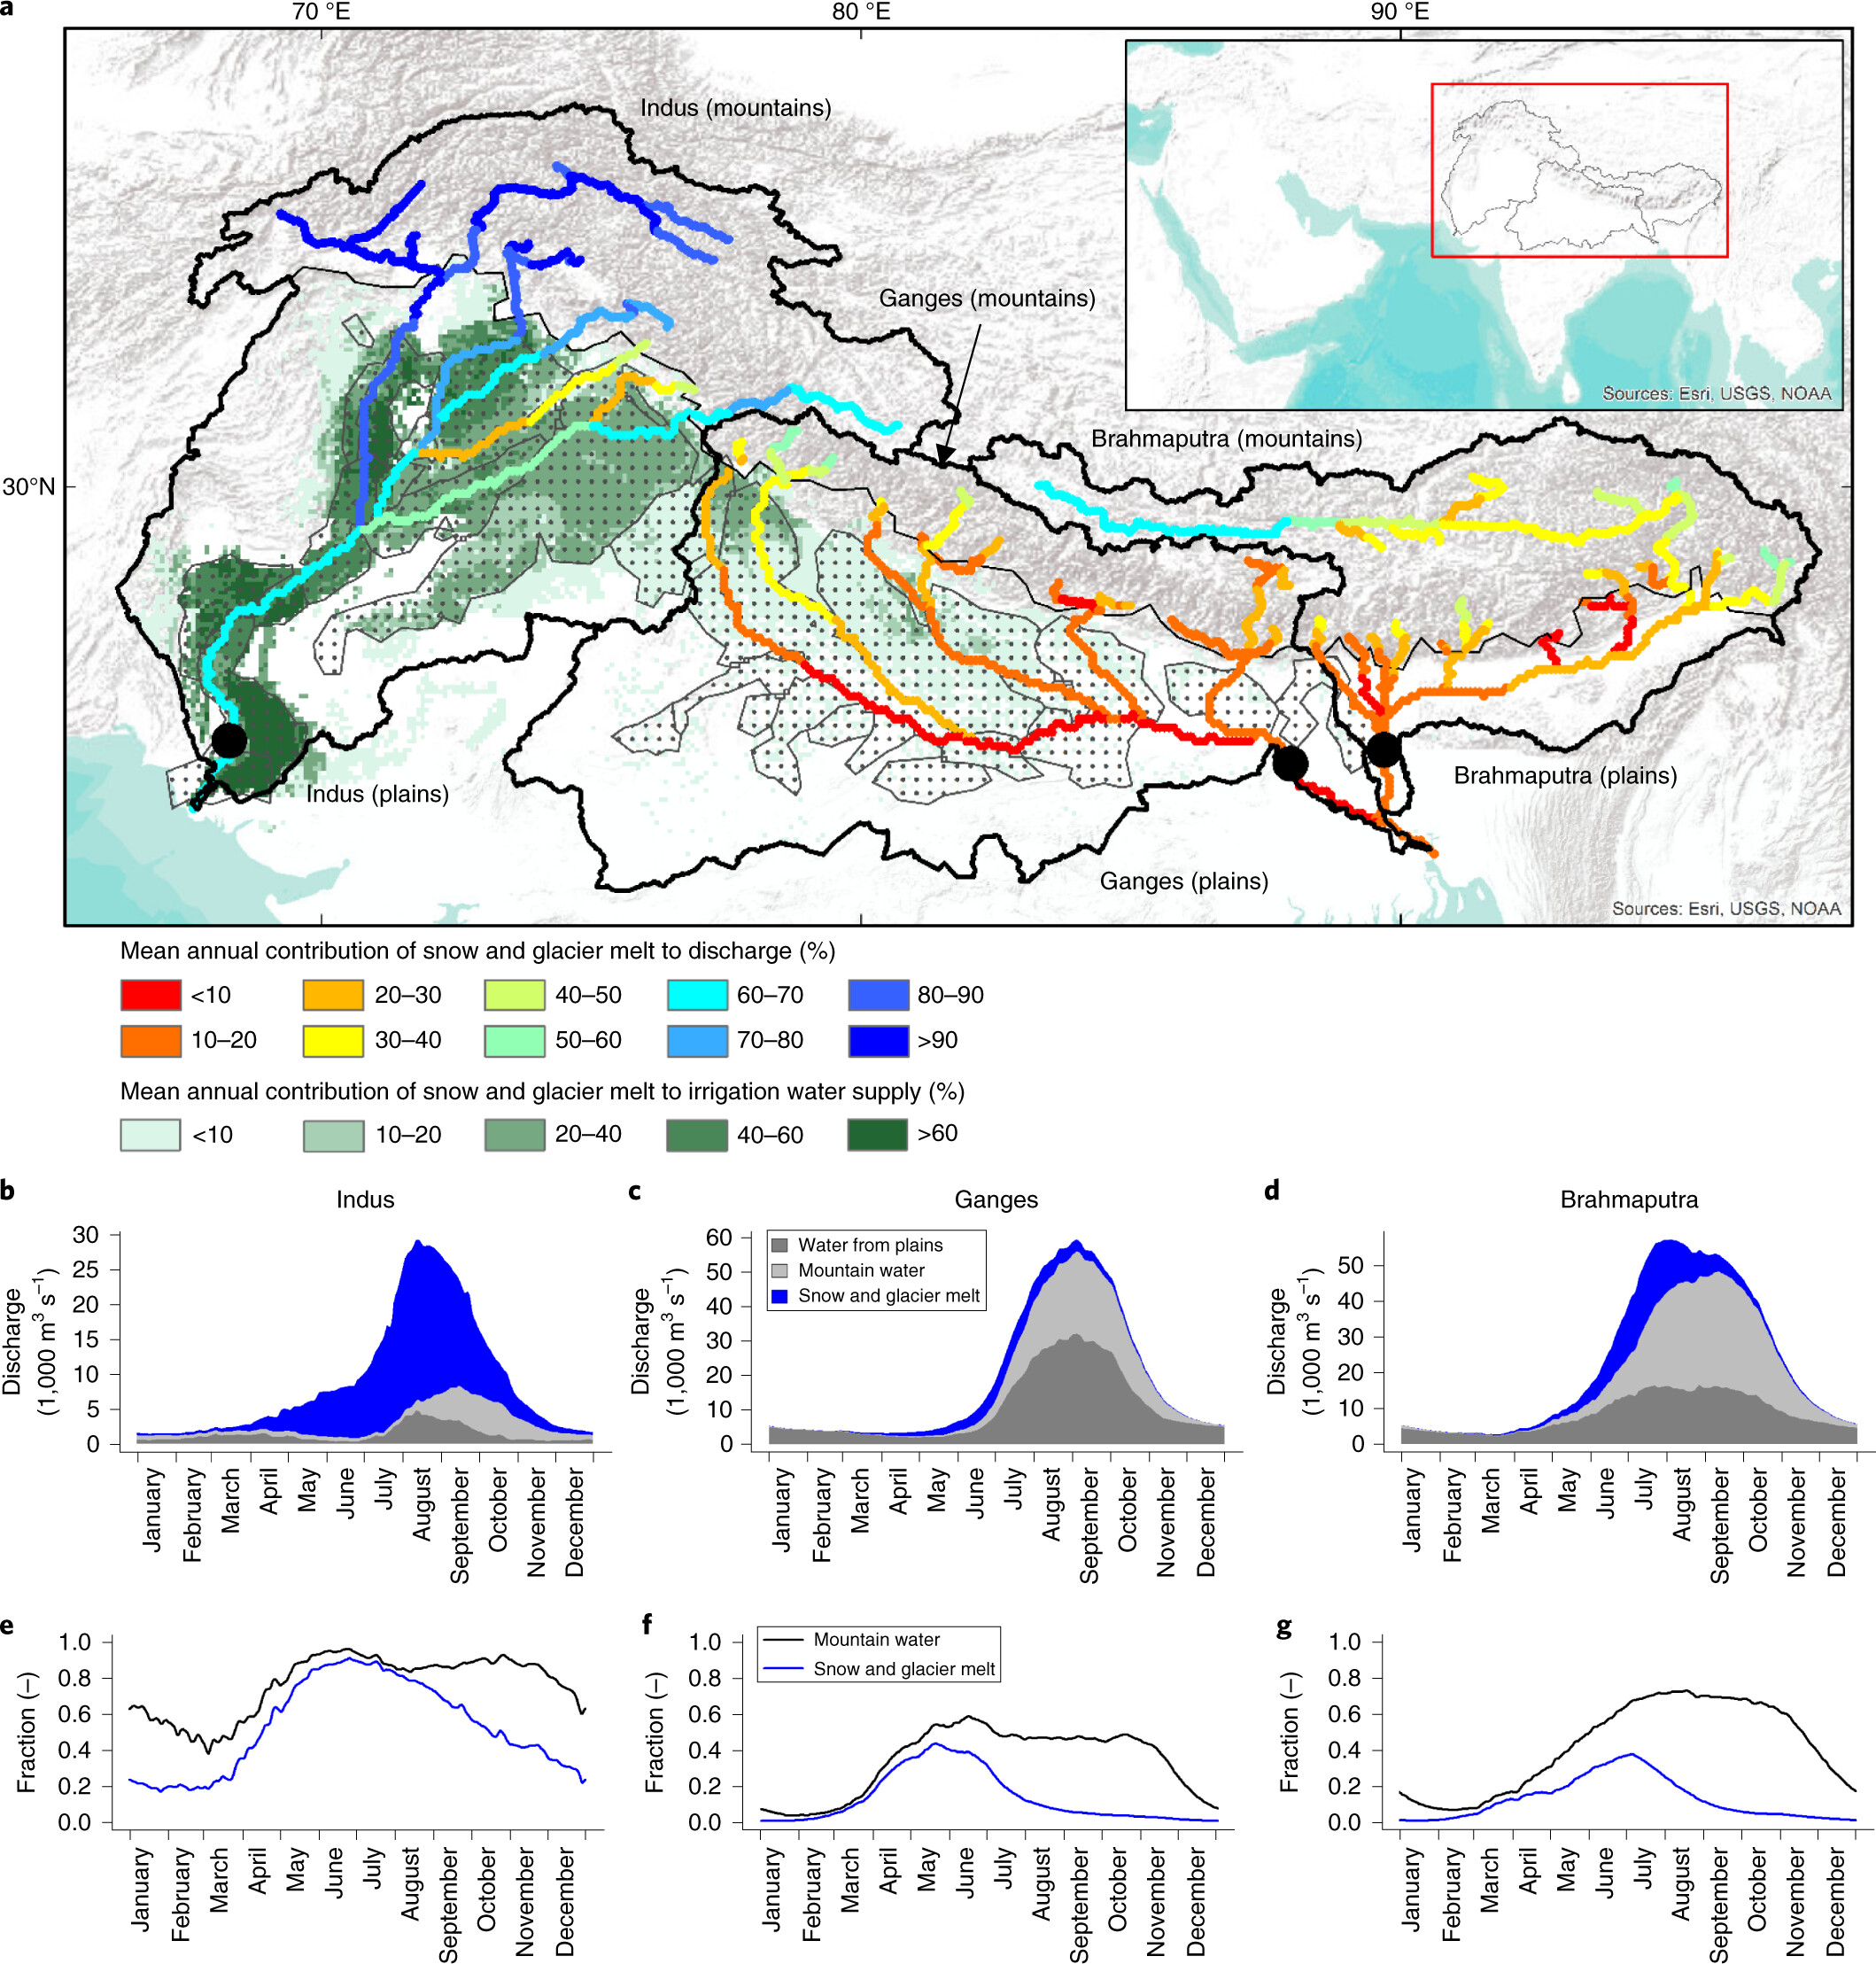
\includegraphics[width=\textwidth]{02-figures/Biemans.png}
    \caption{The spatially explicit, mean annual contributions of snow and glacier melt to river flow from \citet{biemans2019importance}.}
    \label{figS:Biemans}
\end{figure*}

\newpage 
\clearpage 
%% REFERENCES
\bibliographystyle{copernicus}
\bibliography{reference.bib}


\end{document}
